% Options for packages loaded elsewhere
% Options for packages loaded elsewhere
\PassOptionsToPackage{unicode}{hyperref}
\PassOptionsToPackage{hyphens}{url}
\PassOptionsToPackage{dvipsnames,svgnames,x11names}{xcolor}
%
\documentclass[
  letterpaper,
  DIV=11,
  numbers=noendperiod]{scrreprt}
\usepackage{xcolor}
\usepackage[margin=1in]{geometry}
\usepackage{amsmath,amssymb}
\setcounter{secnumdepth}{5}
\usepackage{iftex}
\ifPDFTeX
  \usepackage[T1]{fontenc}
  \usepackage[utf8]{inputenc}
  \usepackage{textcomp} % provide euro and other symbols
\else % if luatex or xetex
  \usepackage{unicode-math} % this also loads fontspec
  \defaultfontfeatures{Scale=MatchLowercase}
  \defaultfontfeatures[\rmfamily]{Ligatures=TeX,Scale=1}
\fi
\usepackage{lmodern}
\ifPDFTeX\else
  % xetex/luatex font selection
  \setmainfont[]{Noto Serif CJK KR}
  \setmonofont[]{Noto Sans Mono CJK KR}
\fi
% Use upquote if available, for straight quotes in verbatim environments
\IfFileExists{upquote.sty}{\usepackage{upquote}}{}
\IfFileExists{microtype.sty}{% use microtype if available
  \usepackage[]{microtype}
  \UseMicrotypeSet[protrusion]{basicmath} % disable protrusion for tt fonts
}{}
\makeatletter
\@ifundefined{KOMAClassName}{% if non-KOMA class
  \IfFileExists{parskip.sty}{%
    \usepackage{parskip}
  }{% else
    \setlength{\parindent}{0pt}
    \setlength{\parskip}{6pt plus 2pt minus 1pt}}
}{% if KOMA class
  \KOMAoptions{parskip=half}}
\makeatother
% Make \paragraph and \subparagraph free-standing
\makeatletter
\ifx\paragraph\undefined\else
  \let\oldparagraph\paragraph
  \renewcommand{\paragraph}{
    \@ifstar
      \xxxParagraphStar
      \xxxParagraphNoStar
  }
  \newcommand{\xxxParagraphStar}[1]{\oldparagraph*{#1}\mbox{}}
  \newcommand{\xxxParagraphNoStar}[1]{\oldparagraph{#1}\mbox{}}
\fi
\ifx\subparagraph\undefined\else
  \let\oldsubparagraph\subparagraph
  \renewcommand{\subparagraph}{
    \@ifstar
      \xxxSubParagraphStar
      \xxxSubParagraphNoStar
  }
  \newcommand{\xxxSubParagraphStar}[1]{\oldsubparagraph*{#1}\mbox{}}
  \newcommand{\xxxSubParagraphNoStar}[1]{\oldsubparagraph{#1}\mbox{}}
\fi
\makeatother

\usepackage{color}
\usepackage{fancyvrb}
\newcommand{\VerbBar}{|}
\newcommand{\VERB}{\Verb[commandchars=\\\{\}]}
\DefineVerbatimEnvironment{Highlighting}{Verbatim}{commandchars=\\\{\}}
% Add ',fontsize=\small' for more characters per line
\usepackage{framed}
\definecolor{shadecolor}{RGB}{241,243,245}
\newenvironment{Shaded}{\begin{snugshade}}{\end{snugshade}}
\newcommand{\AlertTok}[1]{\textcolor[rgb]{0.68,0.00,0.00}{#1}}
\newcommand{\AnnotationTok}[1]{\textcolor[rgb]{0.37,0.37,0.37}{#1}}
\newcommand{\AttributeTok}[1]{\textcolor[rgb]{0.40,0.45,0.13}{#1}}
\newcommand{\BaseNTok}[1]{\textcolor[rgb]{0.68,0.00,0.00}{#1}}
\newcommand{\BuiltInTok}[1]{\textcolor[rgb]{0.00,0.23,0.31}{#1}}
\newcommand{\CharTok}[1]{\textcolor[rgb]{0.13,0.47,0.30}{#1}}
\newcommand{\CommentTok}[1]{\textcolor[rgb]{0.37,0.37,0.37}{#1}}
\newcommand{\CommentVarTok}[1]{\textcolor[rgb]{0.37,0.37,0.37}{\textit{#1}}}
\newcommand{\ConstantTok}[1]{\textcolor[rgb]{0.56,0.35,0.01}{#1}}
\newcommand{\ControlFlowTok}[1]{\textcolor[rgb]{0.00,0.23,0.31}{\textbf{#1}}}
\newcommand{\DataTypeTok}[1]{\textcolor[rgb]{0.68,0.00,0.00}{#1}}
\newcommand{\DecValTok}[1]{\textcolor[rgb]{0.68,0.00,0.00}{#1}}
\newcommand{\DocumentationTok}[1]{\textcolor[rgb]{0.37,0.37,0.37}{\textit{#1}}}
\newcommand{\ErrorTok}[1]{\textcolor[rgb]{0.68,0.00,0.00}{#1}}
\newcommand{\ExtensionTok}[1]{\textcolor[rgb]{0.00,0.23,0.31}{#1}}
\newcommand{\FloatTok}[1]{\textcolor[rgb]{0.68,0.00,0.00}{#1}}
\newcommand{\FunctionTok}[1]{\textcolor[rgb]{0.28,0.35,0.67}{#1}}
\newcommand{\ImportTok}[1]{\textcolor[rgb]{0.00,0.46,0.62}{#1}}
\newcommand{\InformationTok}[1]{\textcolor[rgb]{0.37,0.37,0.37}{#1}}
\newcommand{\KeywordTok}[1]{\textcolor[rgb]{0.00,0.23,0.31}{\textbf{#1}}}
\newcommand{\NormalTok}[1]{\textcolor[rgb]{0.00,0.23,0.31}{#1}}
\newcommand{\OperatorTok}[1]{\textcolor[rgb]{0.37,0.37,0.37}{#1}}
\newcommand{\OtherTok}[1]{\textcolor[rgb]{0.00,0.23,0.31}{#1}}
\newcommand{\PreprocessorTok}[1]{\textcolor[rgb]{0.68,0.00,0.00}{#1}}
\newcommand{\RegionMarkerTok}[1]{\textcolor[rgb]{0.00,0.23,0.31}{#1}}
\newcommand{\SpecialCharTok}[1]{\textcolor[rgb]{0.37,0.37,0.37}{#1}}
\newcommand{\SpecialStringTok}[1]{\textcolor[rgb]{0.13,0.47,0.30}{#1}}
\newcommand{\StringTok}[1]{\textcolor[rgb]{0.13,0.47,0.30}{#1}}
\newcommand{\VariableTok}[1]{\textcolor[rgb]{0.07,0.07,0.07}{#1}}
\newcommand{\VerbatimStringTok}[1]{\textcolor[rgb]{0.13,0.47,0.30}{#1}}
\newcommand{\WarningTok}[1]{\textcolor[rgb]{0.37,0.37,0.37}{\textit{#1}}}

\usepackage{longtable,booktabs,array}
\newcounter{none} % for unnumbered tables
\usepackage{calc} % for calculating minipage widths
% Correct order of tables after \paragraph or \subparagraph
\usepackage{etoolbox}
\makeatletter
\patchcmd\longtable{\par}{\if@noskipsec\mbox{}\fi\par}{}{}
\makeatother
% Allow footnotes in longtable head/foot
\IfFileExists{footnotehyper.sty}{\usepackage{footnotehyper}}{\usepackage{footnote}}
\makesavenoteenv{longtable}
\usepackage{graphicx}
\makeatletter
\newsavebox\pandoc@box
\newcommand*\pandocbounded[1]{% scales image to fit in text height/width
  \sbox\pandoc@box{#1}%
  \Gscale@div\@tempa{\textheight}{\dimexpr\ht\pandoc@box+\dp\pandoc@box\relax}%
  \Gscale@div\@tempb{\linewidth}{\wd\pandoc@box}%
  \ifdim\@tempb\p@<\@tempa\p@\let\@tempa\@tempb\fi% select the smaller of both
  \ifdim\@tempa\p@<\p@\scalebox{\@tempa}{\usebox\pandoc@box}%
  \else\usebox{\pandoc@box}%
  \fi%
}
% Set default figure placement to htbp
\def\fps@figure{htbp}
\makeatother





\setlength{\emergencystretch}{3em} % prevent overfull lines

\providecommand{\tightlist}{%
  \setlength{\itemsep}{0pt}\setlength{\parskip}{0pt}}



 


\usepackage{amsmath,amssymb,bm}
\KOMAoption{captions}{tableheading}
\makeatletter
\@ifpackageloaded{tcolorbox}{}{\usepackage[skins,breakable]{tcolorbox}}
\@ifpackageloaded{fontawesome5}{}{\usepackage{fontawesome5}}
\definecolor{quarto-callout-color}{HTML}{909090}
\definecolor{quarto-callout-note-color}{HTML}{0758E5}
\definecolor{quarto-callout-important-color}{HTML}{CC1914}
\definecolor{quarto-callout-warning-color}{HTML}{EB9113}
\definecolor{quarto-callout-tip-color}{HTML}{00A047}
\definecolor{quarto-callout-caution-color}{HTML}{FC5300}
\definecolor{quarto-callout-color-frame}{HTML}{acacac}
\definecolor{quarto-callout-note-color-frame}{HTML}{4582ec}
\definecolor{quarto-callout-important-color-frame}{HTML}{d9534f}
\definecolor{quarto-callout-warning-color-frame}{HTML}{f0ad4e}
\definecolor{quarto-callout-tip-color-frame}{HTML}{02b875}
\definecolor{quarto-callout-caution-color-frame}{HTML}{fd7e14}
\makeatother
\makeatletter
\@ifpackageloaded{caption}{}{\usepackage{caption}}
\AtBeginDocument{%
\ifdefined\contentsname
  \renewcommand*\contentsname{Table of contents}
\else
  \newcommand\contentsname{Table of contents}
\fi
\ifdefined\listfigurename
  \renewcommand*\listfigurename{List of Figures}
\else
  \newcommand\listfigurename{List of Figures}
\fi
\ifdefined\listtablename
  \renewcommand*\listtablename{List of Tables}
\else
  \newcommand\listtablename{List of Tables}
\fi
\ifdefined\figurename
  \renewcommand*\figurename{Figure}
\else
  \newcommand\figurename{Figure}
\fi
\ifdefined\tablename
  \renewcommand*\tablename{Table}
\else
  \newcommand\tablename{Table}
\fi
}
\@ifpackageloaded{float}{}{\usepackage{float}}
\floatstyle{ruled}
\@ifundefined{c@chapter}{\newfloat{codelisting}{h}{lop}}{\newfloat{codelisting}{h}{lop}[chapter]}
\floatname{codelisting}{Listing}
\newcommand*\listoflistings{\listof{codelisting}{List of Listings}}
\makeatother
\makeatletter
\makeatother
\makeatletter
\@ifpackageloaded{caption}{}{\usepackage{caption}}
\@ifpackageloaded{subcaption}{}{\usepackage{subcaption}}
\makeatother
\usepackage{bookmark}
\IfFileExists{xurl.sty}{\usepackage{xurl}}{} % add URL line breaks if available
\urlstyle{same}
\hypersetup{
  pdftitle={Regularization for Deep Learning},
  colorlinks=true,
  linkcolor={blue},
  filecolor={Maroon},
  citecolor={Blue},
  urlcolor={Blue},
  pdfcreator={LaTeX via pandoc}}


\title{Regularization for Deep Learning}
\usepackage{etoolbox}
\makeatletter
\providecommand{\subtitle}[1]{% add subtitle to \maketitle
  \apptocmd{\@title}{\par {\large #1 \par}}{}{}
}
\makeatother
\subtitle{딥러닝의 9가지 정규화 기법 --- 수학적 유도와 직관}
\author{}
\date{2026-04-12}
\begin{document}
\maketitle

\renewcommand*\contentsname{Table of contents}
{
\setcounter{tocdepth}{2}
\tableofcontents
}

\chapter{정규화의 큰 그림}\label{sec-overview}

\section{한 줄 요약}\label{uxd55c-uxc904-uxc694uxc57d}

\begin{quote}
\textbf{정규화(Regularization)란 ``훈련 오차를 늘리더라도 일반화
오차(generalization error)를 줄이려는 모든 수정''을 말한다.}
본질적으로는 모델에 \textbf{귀납적 편향(inductive bias)}, 즉
``데이터만으로는 결정할 수 없는 부분에 대한 우리의 사전 믿음''을
주입하는 행위다.
\end{quote}

\section{왜 필요한가: 편향-분산
분해}\label{uxc65c-uxd544uxc694uxd55cuxac00-uxd3b8uxd5a5-uxbd84uxc0b0-uxbd84uxd574}

유한한 데이터 \(\mathcal{D}=\{(\bm{x}_i,y_i)\}_{i=1}^N\) 로 학습한
추정량 \(\hat{f}_\mathcal{D}\) 의 기대 제곱 오차는 다음처럼 분해된다.

\begin{equation}\protect\phantomsection\label{eq-bias-var}{
\underbrace{\mathbb{E}_{\mathcal{D}}\!\left[(\hat{f}_\mathcal{D}(\bm{x}) - f^*(\bm{x}))^2\right]}_{\text{기대 오차}}
= \underbrace{\left(\mathbb{E}_\mathcal{D}[\hat{f}_\mathcal{D}(\bm{x})] - f^*(\bm{x})\right)^2}_{\text{Bias}^2}
+ \underbrace{\mathbb{E}_\mathcal{D}\!\left[(\hat{f}_\mathcal{D}(\bm{x}) - \mathbb{E}_\mathcal{D}[\hat{f}_\mathcal{D}(\bm{x})])^2\right]}_{\text{Variance}}
}\end{equation}

심층 신경망은 표현력(capacity)이 커서 \textbf{분산이 지배적인 영역}에서
동작하기 쉽다. 정규화는 약간의 편향을 받아들이는 대신 분산을 크게 깎아
식~\ref{eq-bias-var} 의 총합을 낮춘다.

\begin{tcolorbox}[enhanced jigsaw, arc=.35mm, bottomrule=.15mm, bottomtitle=1mm, breakable, colback=white, colbacktitle=quarto-callout-note-color!10!white, colframe=quarto-callout-note-color-frame, coltitle=black, left=2mm, leftrule=.75mm, opacityback=0, opacitybacktitle=0.6, rightrule=.15mm, title=\textcolor{quarto-callout-note-color}{\faInfo}\hspace{0.5em}{통계적 추론 관점}, titlerule=0mm, toprule=.15mm, toptitle=1mm]

정규화는 ill-posed 역문제(inverse problem)를 well-posed로 바꾸는 작업과
동형이다. 무선통신에서 안테나 수보다 추정해야 할 경로(path)가 많을
때(under-determined), 채널이 \textbf{희소(sparse)}하다는 사전지식을
\(\ell_1\) 페널티로 넣어 해를 유일하게 만드는 것 --- 이것이 바로
compressed sensing이며, 정규화의 전형적 사례다.

\end{tcolorbox}

\section{정규화의 세 가지
형식}\label{uxc815uxaddcuxd654uxc758-uxc138-uxac00uxc9c0-uxd615uxc2dd}

학습 목적함수는 보편적으로 다음 형태를 갖는다.

\begin{equation}\protect\phantomsection\label{eq-objective}{
\min_{\bm{\theta}} \; \underbrace{L(\bm{\theta};\mathcal{D})}_{\text{Loss: 최적화 대상}} + \underbrace{\Omega(\bm{\theta})}_{\text{Regularizer: 귀납적 편향}}
}\end{equation}

손쉽게 만든(hand-crafted) 정규화는 세 가지 관점으로 통일된다.

{\def\LTcaptype{none} % do not increment counter
\begin{longtable}[]{@{}
  >{\raggedright\arraybackslash}p{(\linewidth - 4\tabcolsep) * \real{0.3333}}
  >{\raggedright\arraybackslash}p{(\linewidth - 4\tabcolsep) * \real{0.3333}}
  >{\raggedright\arraybackslash}p{(\linewidth - 4\tabcolsep) * \real{0.3333}}@{}}
\toprule\noalign{}
\begin{minipage}[b]{\linewidth}\raggedright
형식
\end{minipage} & \begin{minipage}[b]{\linewidth}\raggedright
정의
\end{minipage} & \begin{minipage}[b]{\linewidth}\raggedright
대표 예
\end{minipage} \\
\midrule\noalign{}
\endhead
\bottomrule\noalign{}
\endlastfoot
\textbf{Hard constraint} & \(\min_{\bm{\theta}} L(\bm{\theta})\) s.t.
\(R(\bm{\theta}) \le c\) & 가중치 노름 상한 제약 \\
\textbf{Soft constraint} &
\(\min_{\bm{\theta}} L(\bm{\theta}) + \lambda R(\bm{\theta})\) &
\(\ell_2\) weight decay, \(\ell_1\) \\
\textbf{Bayesian prior} & 사후확률 최대화(MAP) & prior
\(p(\bm{\theta})\) 도입 \\
\end{longtable}
}

\subsection{Hard constraint와 Soft constraint의
등가성}\label{hard-constraintuxc640-soft-constraintuxc758-uxb4f1uxac00uxc131}

하드 제약 문제

\[
\bm{\theta}^* = \arg\min_{\bm{\theta}} L(\bm{\theta}) \quad \text{s.t.}\quad R(\bm{\theta}) \le c
\]

의 KKT 조건을 쓰면, 어떤 \(\lambda^* > 0\) 에 대해

\[
\bm{\theta}^* = \arg\min_{\bm{\theta}} \; L(\bm{\theta}) + \lambda^*\big(R(\bm{\theta}) - c\big)
\]

가 성립한다. 상수 \(-\lambda^* c\) 는 \(\bm{\theta}\) 에 무관하므로
제거되고, 결국 \textbf{하드 제약 = 소프트 제약}이 된다. \(c\) 가
작을수록(강한 제약) 대응하는 \(\lambda^*\) 는 커진다.

\subsection{Bayesian prior로서의 정규화: MAP = MLE + log
prior}\label{bayesian-prioruxb85cuxc11cuxc758-uxc815uxaddcuxd654-map-mle-log-prior}

베이즈 정리

\[
p(\bm{\theta}\mid\mathcal{D}) = \frac{p(\bm{\theta})\,p(\mathcal{D}\mid\bm{\theta})}{p(\mathcal{D})}
\]

에서 사후확률을 최대화(MAP)하면, \(p(\mathcal{D})\) 는 \(\bm{\theta}\)
와 무관하므로

\begin{equation}\protect\phantomsection\label{eq-map}{
\bm{\theta}_{\text{MAP}}
= \arg\max_{\bm{\theta}} \underbrace{\log p(\mathcal{D}\mid\bm{\theta})}_{\text{MLE loss}} + \underbrace{\log p(\bm{\theta})}_{\text{Regularizer}}
}\end{equation}

\begin{tcolorbox}[enhanced jigsaw, arc=.35mm, bottomrule=.15mm, bottomtitle=1mm, breakable, colback=white, colbacktitle=quarto-callout-important-color!10!white, colframe=quarto-callout-important-color-frame, coltitle=black, left=2mm, leftrule=.75mm, opacityback=0, opacitybacktitle=0.6, rightrule=.15mm, title=\textcolor{quarto-callout-important-color}{\faExclamation}\hspace{0.5em}{정확한 진술 (자주 틀리는 부분)}, titlerule=0mm, toprule=.15mm, toptitle=1mm]

\begin{itemize}
\tightlist
\item
  \textbf{MAP = MLE + log-prior 정규화항.} MLE는 prior를 ``무시''하는
  것이 아니라 \textbf{균일 사전분포(uniform prior)를 가정}한 MAP의
  특수경우다.
\item
  \(\ell_2\) 정규화 \(\Leftrightarrow\) 가우시안 prior
  \(p(\bm{\theta})=\mathcal{N}(\bm{0},\sigma^2 I)\) 의 MAP.
\item
  \(\ell_1\) 정규화 \(\Leftrightarrow\) 라플라스(Laplace) prior의 MAP
  \(\to\) 희소성(sparsity) 유도.
\item
  \(\ell_0\) 페널티는 비영(non-zero) 원소 개수를 직접 세므로 희소성을
  \textbf{강제}하지만 비볼록·NP-hard.
\end{itemize}

\end{tcolorbox}

이제 이 틀 위에서, 심층학습에서 실제로 널리 쓰이는 \textbf{9가지 정규화
기법}을 하나씩 본다. 각 기법이 식~\ref{eq-objective} 의 어느 항을 어떻게
건드리는지에 주목하라.

\begin{center}\rule{0.5\linewidth}{0.5pt}\end{center}

\chapter{Dataset Augmentation}\label{sec-augment}

\section{핵심}\label{uxd575uxc2ec}

\begin{quote}
\textbf{레이블을 보존하는 변환(label-preserving transformation)으로 훈련
데이터를 인위적으로 늘려, 모델이 그 변환에 대해 불변(invariant)하도록
만든다.} ``더 많은 진짜 데이터를 못 구한다면, 가짜를 합성하라.''
\end{quote}

\section{형식화}\label{uxd615uxc2dduxd654}

변환 분포 \(T(\cdot\mid\bm{x})\) (예: 회전, 이동, 색 변형)에 대해 손실을
변환된 입력의 기댓값으로 바꾼다.

\begin{equation}\protect\phantomsection\label{eq-aug}{
\tilde{L}(\bm{\theta}) = \mathbb{E}_{(\bm{x},y)\sim\mathcal{D}}\;\mathbb{E}_{\tilde{\bm{x}}\sim T(\cdot\mid\bm{x})}\big[\ell\big(f_{\bm{\theta}}(\tilde{\bm{x}}),\,y\big)\big]
}\end{equation}

이는 데이터 분포를 변환 궤도(orbit)를 따라 ``퍼뜨려'' 결정 경계를
매끄럽게 만드는 효과를 준다.

\begin{tcolorbox}[enhanced jigsaw, arc=.35mm, bottomrule=.15mm, bottomtitle=1mm, breakable, colback=white, colbacktitle=quarto-callout-tip-color!10!white, colframe=quarto-callout-tip-color-frame, coltitle=black, left=2mm, leftrule=.75mm, opacityback=0, opacitybacktitle=0.6, rightrule=.15mm, title=\textcolor{quarto-callout-tip-color}{\faLightbulb}\hspace{0.5em}{노이즈 주입 = \(\ell_2\) 정규화 (소량 가우시안의 경우)}, titlerule=0mm, toprule=.15mm, toptitle=1mm]

입력에 작은 가우시안 노이즈
\(\tilde{\bm{x}}=\bm{x}+\bm{\epsilon},\ \bm{\epsilon}\sim\mathcal{N}(\bm{0},\sigma^2 I)\)
를 더하고 회귀 손실을 2차 테일러 전개하면, 그 기댓값은 대략

\[
\mathbb{E}_{\bm{\epsilon}}[\ell] \approx \ell(\bm{x}) + \tfrac{\sigma^2}{2}\,\mathbb{E}\big[\|\nabla_{\bm{x}} f(\bm{x})\|^2\big]
\]

가 되어, \textbf{자코비안 노름에 대한 페널티}(함수의 평탄성 유도)로
작동한다. 즉 데이터 증강은 암묵적 정규화항을 추가하는 것과 같다.

\end{tcolorbox}

\section{직관과 주의점}\label{uxc9c1uxad00uxacfc-uxc8fcuxc758uxc810}

\begin{itemize}
\tightlist
\item
  변환은 반드시 \textbf{레이블 불변}이어야 한다. 손글씨 '6'을 180°
  회전하면 '9'가 되므로 회전 증강은 위험하다.
\item
  도메인 지식이 곧 좋은 증강을 결정한다 --- 이것이 증강을 ``수작업 귀납
  편향''이라 부르는 이유다.
\end{itemize}

\begin{tcolorbox}[enhanced jigsaw, arc=.35mm, bottomrule=.15mm, bottomtitle=1mm, breakable, colback=white, colbacktitle=quarto-callout-note-color!10!white, colframe=quarto-callout-note-color-frame, coltitle=black, left=2mm, leftrule=.75mm, opacityback=0, opacitybacktitle=0.6, rightrule=.15mm, title=\textcolor{quarto-callout-note-color}{\faInfo}\hspace{0.5em}{무선통신 비유}, titlerule=0mm, toprule=.15mm, toptitle=1mm]

이퀄라이저/수신기를 \textbf{여러 채널 실현(channel realization)에 대해
훈련}하는 것과 동일하다. 페이딩 채널을 Monte-Carlo로 샘플링해 다양한
\(\bm{h}\) 하에서 학습시키면, 수신기가 특정 채널에 과적합하지 않고 채널
분포 전체에 강인해진다. 식 식~\ref{eq-aug} 의 \(T\) 가 곧 채널 분포
\(p(\bm{h})\) 다.

\end{tcolorbox}

\begin{center}\rule{0.5\linewidth}{0.5pt}\end{center}

\chapter{Adversarial Examples}\label{sec-adv}

\section{핵심}\label{uxd575uxc2ec-1}

\begin{quote}
\textbf{사람 눈엔 거의 동일하지만 모델을 속이는 미세 섭동(adversarial
perturbation)을 일부러 만들어 함께 학습시킨다.} 주목적은
보안(robustness)이지만, \textbf{결정 경계를 입력 변화에 둔감하게} 만들어
일반화에도 도움을 준다.
\end{quote}

\section{적대적 예제 생성:
FGSM}\label{uxc801uxb300uxc801-uxc608uxc81c-uxc0dduxc131-fgsm}

손실 \(J(\bm{\theta},\bm{x},y)\) 를 입력에 대해 1차 선형화하면,
\(\ell_\infty\) 제약 하에서 손실을 가장 키우는 섭동은 그래디언트의
부호다 (Fast Gradient Sign Method).

\begin{equation}\protect\phantomsection\label{eq-fgsm}{
\bm{x}_{\text{adv}} = \bm{x} + \epsilon \cdot \mathrm{sign}\big(\nabla_{\bm{x}} J(\bm{\theta},\bm{x},y)\big)
}\end{equation}

고차원에서는 아주 작은 \(\epsilon\) 의 섭동도 수많은 차원에 걸쳐
누적되어 출력을 크게 흔든다(선형성 가설). 판다 이미지에 사람 눈에 보이지
않는 섭동을 더해 긴팔원숭이로 99\% 확신을 갖고 오분류하게 만드는 고전적
사례가 이를 잘 보여준다.

\section{두 가지 학습
전략}\label{uxb450-uxac00uxc9c0-uxd559uxc2b5-uxc804uxb7b5}

\begin{enumerate}
\def\labelenumi{\arabic{enumi}.}
\item
  \textbf{입력에 섭동 주입 (Adversarial training):} 식~\ref{eq-fgsm} 의
  \(\bm{x}_{\text{adv}}\) 를 훈련셋에 추가. minimax 형태로 쓰면

  \[
  \min_{\bm{\theta}}\ \mathbb{E}_{(\bm{x},y)}\Big[\max_{\|\bm{\delta}\|\le\epsilon} J(\bm{\theta},\bm{x}+\bm{\delta},y)\Big]
  \]

  --- \textbf{최악의 경우(worst-case)에 대한 강건 최적화}다.
\item
  \textbf{출력 타깃에 노이즈 주입 (Label smoothing):} 원-핫 타깃을
  부드럽게 만든다. 클래스 수 \(k\), 작은 \(\epsilon\) 에 대해

  \begin{equation}\protect\phantomsection\label{eq-labelsmooth}{
  y_c^{\text{smooth}} =
  \begin{cases}
  1-\epsilon & (\text{정답 클래스}) \\[4pt]
  \dfrac{\epsilon}{k-1} & (\text{나머지 클래스})
  \end{cases}
  }\end{equation}

  소프트맥스가 무한대 로짓으로 폭주하는 것을 막고(과신 방지), 확신이 큰
  예측에서의 그래디언트 소실을 완화한다.
\end{enumerate}

\begin{tcolorbox}[enhanced jigsaw, arc=.35mm, bottomrule=.15mm, bottomtitle=1mm, breakable, colback=white, colbacktitle=quarto-callout-note-color!10!white, colframe=quarto-callout-note-color-frame, coltitle=black, left=2mm, leftrule=.75mm, opacityback=0, opacitybacktitle=0.6, rightrule=.15mm, title=\textcolor{quarto-callout-note-color}{\faInfo}\hspace{0.5em}{무선통신 비유}, titlerule=0mm, toprule=.15mm, toptitle=1mm]

minimax 적대적 학습은 \textbf{재밍(jamming)/최악 간섭에 강인한 수신기
설계}와 정확히 같은 구조다. 송신기-재머의 게임에서, 재머가 신호공간 내
최악 방향으로 전력을 쏟을 때도 성능을 보장하도록 설계하는 robust
beamforming이 식~\ref{eq-fgsm} 의 내부 max에 대응한다.

\end{tcolorbox}

\begin{center}\rule{0.5\linewidth}{0.5pt}\end{center}

\chapter{Semi-Supervised Learning}\label{sec-semi}

\section{핵심}\label{uxd575uxc2ec-2}

\begin{quote}
\textbf{레이블된 데이터(소량)와 레이블 없는 데이터(대량)를 결합한다.}
레이블 없는 데이터의 \textbf{분포 \(p(\bm{x})\) 자체가 정규화 정보}가
되어, 결정 경계를 데이터가 조밀한 영역이 아닌 \textbf{저밀도
영역(low-density region)에 놓이도록} 유도한다.
\end{quote}

\section{형식화}\label{uxd615uxc2dduxd654-1}

목적함수는 지도 항과 비지도(정규화) 항의 결합이다.

\[
L = \underbrace{\sum_{(\bm{x}_i,y_i)\in\mathcal{D}_L}\ell(f(\bm{x}_i),y_i)}_{\text{레이블 정보}}
+ \lambda\underbrace{\sum_{\bm{x}_j\in\mathcal{D}_U}\mathcal{R}(f,\bm{x}_j)}_{\text{분포 정보}}
\]

비지도 항 \(\mathcal{R}\) 의 대표적 선택:

\begin{itemize}
\tightlist
\item
  \textbf{일관성 정규화(consistency):}
  \(\mathcal{R}=\|f(\bm{x})-f(\tilde{\bm{x}})\|^2\), 즉 \(\bm{x}\) 와 그
  증강 \(\tilde{\bm{x}}\) 의 예측이 같아야 함 (cluster assumption).
\item
  \textbf{엔트로피 최소화:} \(\mathcal{R}=H(f(\bm{x}))\), 예측이 한
  클래스로 확신을 갖도록 --- 경계를 저밀도 영역으로 밀어냄.
\end{itemize}

\section{두 가지
시나리오}\label{uxb450-uxac00uxc9c0-uxc2dcuxb098uxb9acuxc624}

\begin{itemize}
\tightlist
\item
  레이블·비레이블 데이터가 \textbf{같은 표현 도메인}일 때: 표준 준지도.
\item
  \textbf{다른 표현 도메인}일 때: 공유 표현(shared representation)을
  학습하는 전이/자기지도 방식과 맞닿는다.
\end{itemize}

\begin{tcolorbox}[enhanced jigsaw, arc=.35mm, bottomrule=.15mm, bottomtitle=1mm, breakable, colback=white, colbacktitle=quarto-callout-note-color!10!white, colframe=quarto-callout-note-color-frame, coltitle=black, left=2mm, leftrule=.75mm, opacityback=0, opacitybacktitle=0.6, rightrule=.15mm, title=\textcolor{quarto-callout-note-color}{\faInfo}\hspace{0.5em}{무선통신 비유}, titlerule=0mm, toprule=.15mm, toptitle=1mm]

\textbf{반-블라인드(semi-blind) 채널 추정}과 동형이다. 소수의 파일럿
심볼(=레이블)로 채널을 대략 잡고, 다수의 데이터 심볼의 통계(수신신호
분포, 정상성·유한 알파벳 같은 구조 = 비레이블 분포정보)를 활용해 추정
분산을 줄인다.

\end{tcolorbox}

\begin{center}\rule{0.5\linewidth}{0.5pt}\end{center}

\chapter{Multi-task Learning (MTL)}\label{sec-mtl}

\section{핵심}\label{uxd575uxc2ec-3}

\begin{quote}
\textbf{여러 과제를 하나의 모델로 동시에 학습}하되, 하위 표현
\(\bm{h}^{\text{shared}}\) 를 공유한다. 각 과제가 서로에게
\textbf{데이터 의존적 prior}로 작용하여, 공유 표현이 어느 한 과제에
과적합되지 못하게 막는다.
\end{quote}

\section{구조}\label{uxad6cuxc870}

\begin{Shaded}
\begin{Highlighting}[]
\NormalTok{flowchart BT}
\NormalTok{    x["입력 x"] {-}{-}\textgreater{} hs["h(shared): 공유 표현"]}
\NormalTok{    hs {-}{-}\textgreater{} h1["h(1): 과제1 전용"]}
\NormalTok{    hs {-}{-}\textgreater{} h2["h(2): 과제2 전용"]}
\NormalTok{    hs {-}{-}\textgreater{} h3["h(3): 추가 인자"]}
\NormalTok{    h1 {-}{-}\textgreater{} y1["y(1)"]}
\NormalTok{    h2 {-}{-}\textgreater{} y2["y(2)"]}
\end{Highlighting}
\end{Shaded}

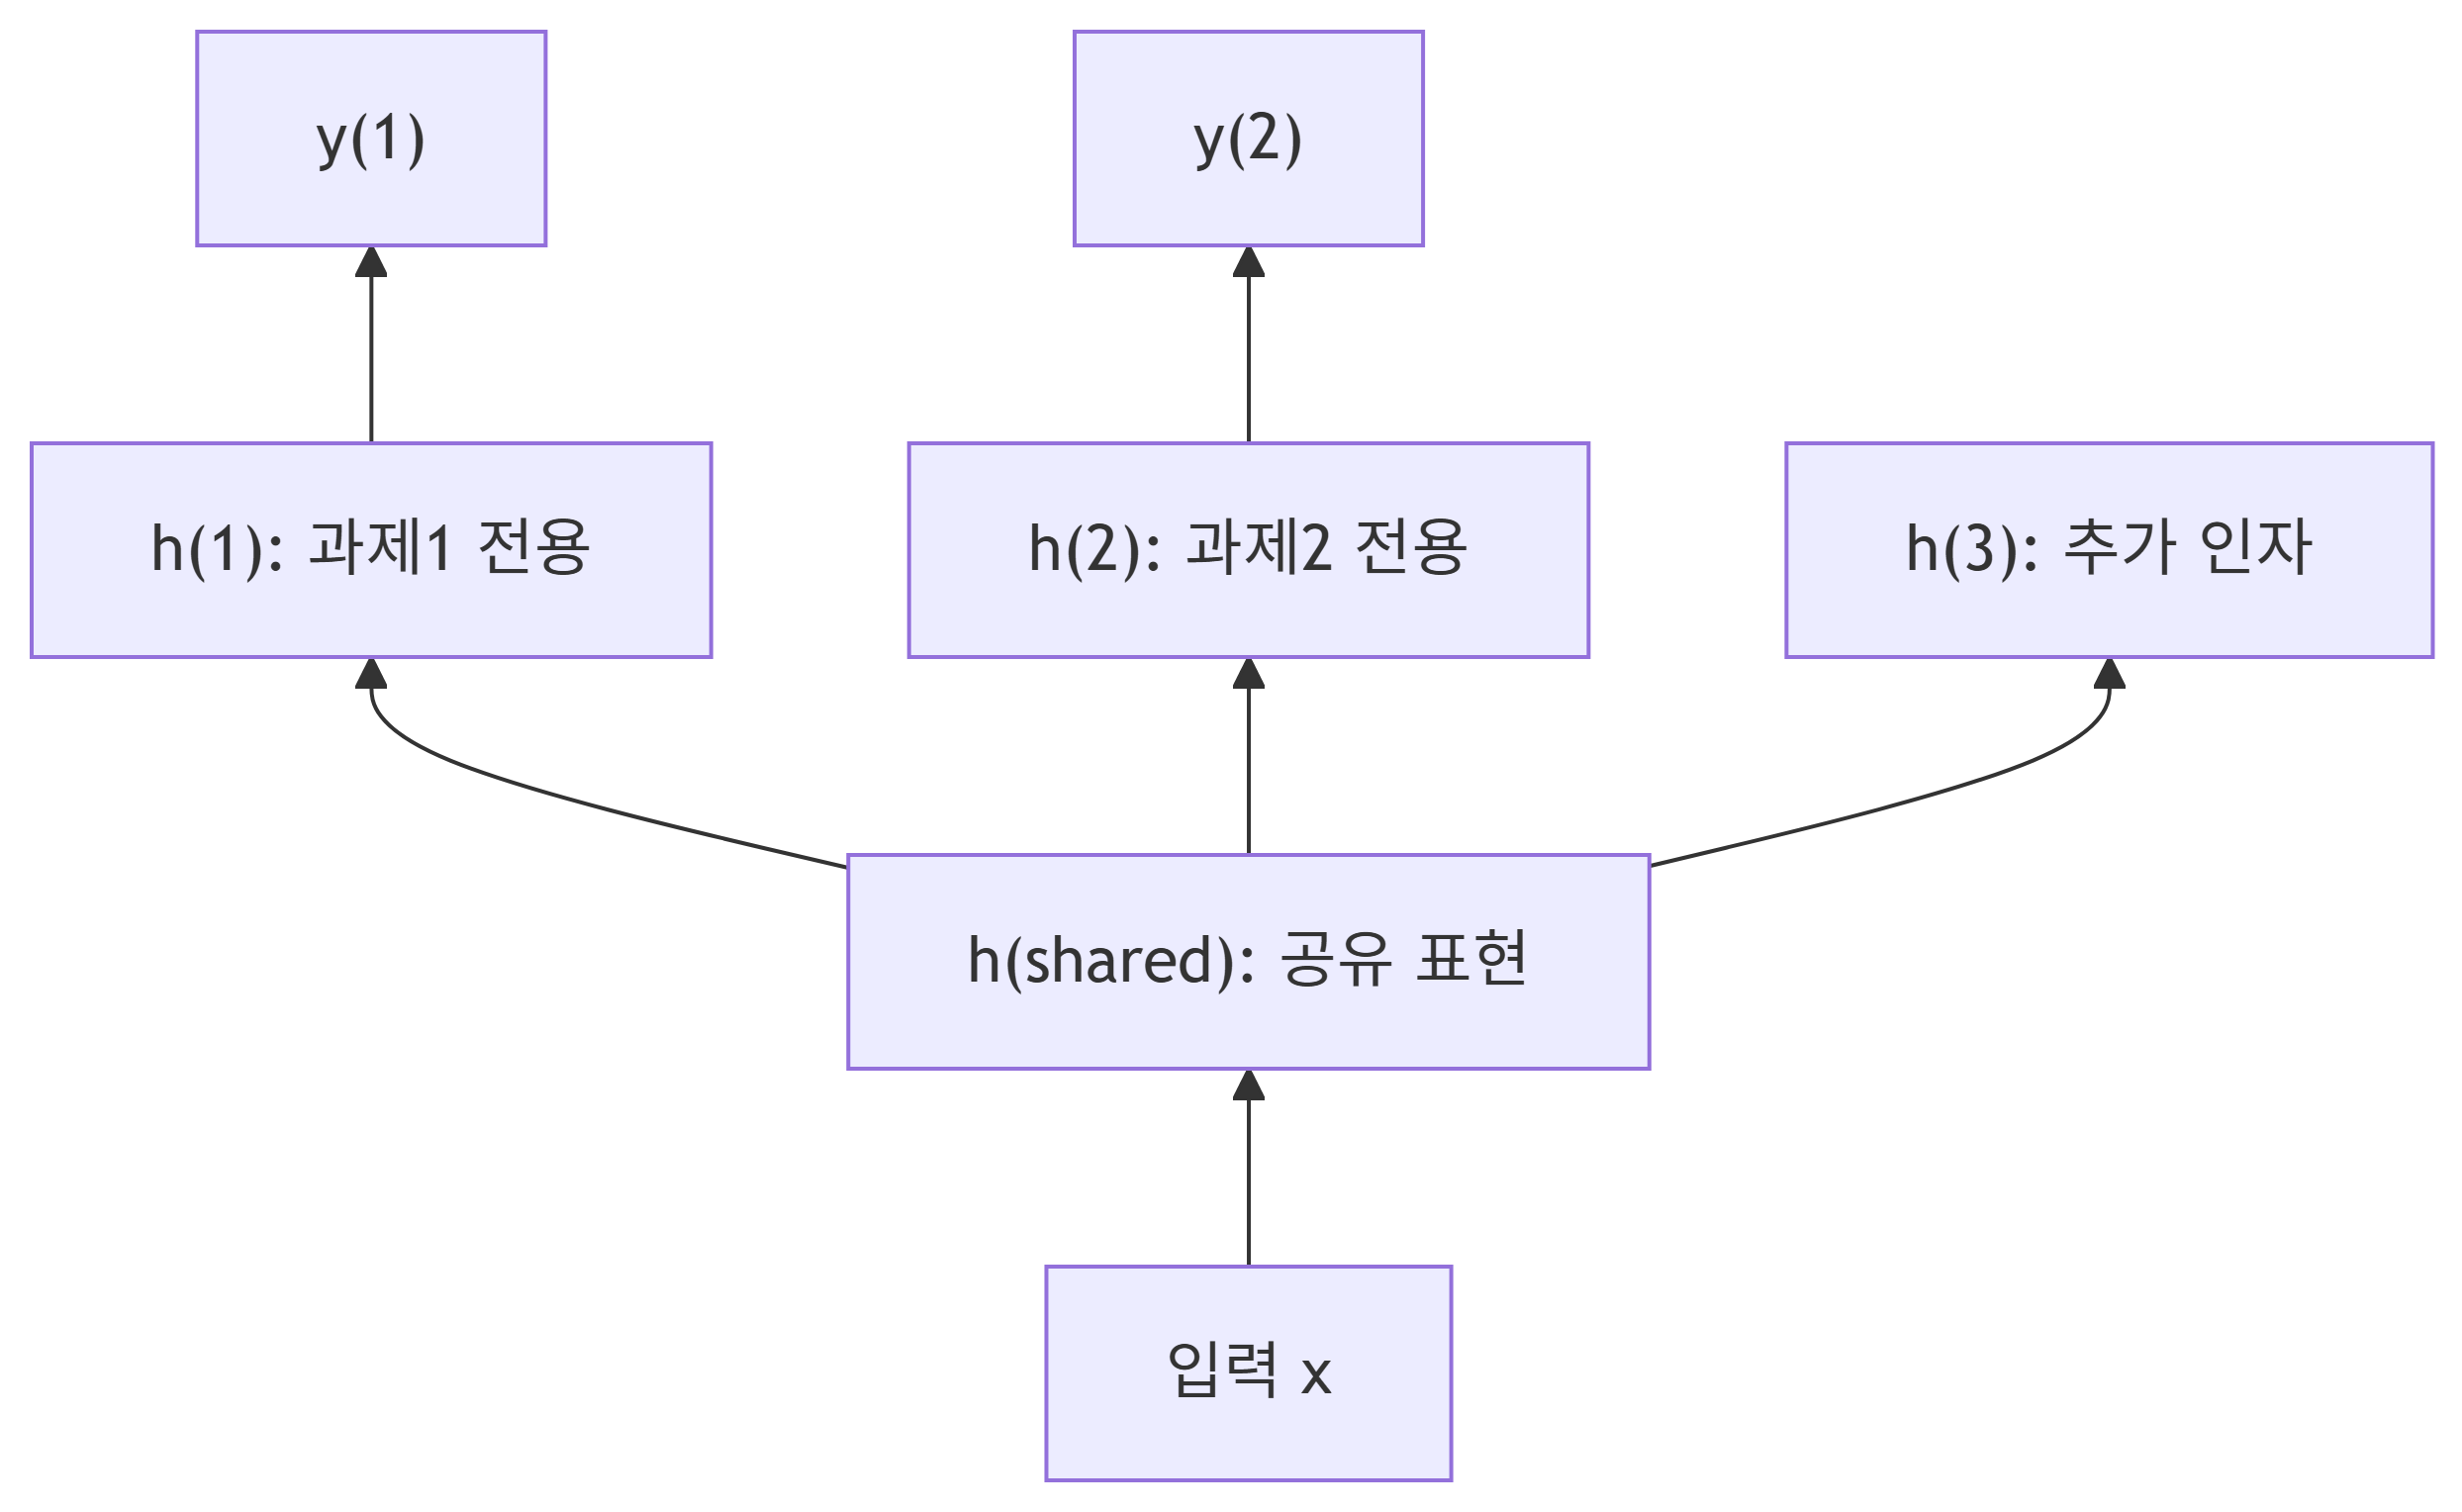
\includegraphics[width=6.49in,height=3.98in]{regularizer-for-dl_files/figure-latex/mermaid-figure-1.png}

목적함수는 과제별 손실의 가중합이다.

\[
L_{\text{MTL}}(\bm{\theta}_{\text{shared}}, \{\bm{\theta}_t\})
= \sum_{t=1}^{T} \alpha_t\, L_t\big(\bm{\theta}_{\text{shared}}, \bm{\theta}_t;\ \mathcal{D}_t\big)
\]

\section{왜 정규화인가}\label{uxc65c-uxc815uxaddcuxd654uxc778uxac00}

공유 파라미터 \(\bm{\theta}_{\text{shared}}\) 는 \textbf{모든 과제의
그래디언트를 동시에 만족}해야 하므로, 탐색 가능한 가설공간이 크게
좁아진다. 이는 식~\ref{eq-objective} 에서 명시적 \(\Omega\) 없이도
\textbf{표현에 부과되는 암묵적 제약}으로 작동한다. 과제들이 공통 잠재
인자(generative factor)를 공유한다는 가정이 성립할수록 효과가 크다.

\begin{tcolorbox}[enhanced jigsaw, arc=.35mm, bottomrule=.15mm, bottomtitle=1mm, breakable, colback=white, colbacktitle=quarto-callout-note-color!10!white, colframe=quarto-callout-note-color-frame, coltitle=black, left=2mm, leftrule=.75mm, opacityback=0, opacitybacktitle=0.6, rightrule=.15mm, title=\textcolor{quarto-callout-note-color}{\faInfo}\hspace{0.5em}{무선통신 비유}, titlerule=0mm, toprule=.15mm, toptitle=1mm]

\textbf{결합 추정(joint estimation)} --- 채널 추정, 주파수 옵셋 보상,
잡음전력 추정을 하나의 수신기가 공통 통계량(공유 표현)을 토대로 동시에
수행하면, 각 추정이 서로를 정규화하여 전체 추정 분산이 줄어든다.

\end{tcolorbox}

\begin{center}\rule{0.5\linewidth}{0.5pt}\end{center}

\chapter{Early Stopping}\label{sec-early}

\section{핵심}\label{uxd575uxc2ec-4}

\begin{quote}
\textbf{검증 오차(validation error)가 더 이상 줄지 않는 시점에서 훈련을
멈춘다.} 가장 흔하고 효율적이며 거의 공짜인 정규화. 훈련을 길게 할수록
모델은 훈련셋에 과적합되므로, 일반화가 최적인 순간을 ``유효
표현력(effective capacity)''을 제어하는 \textbf{하이퍼파라미터}로 삼는
것이다.
\end{quote}

\begin{Shaded}
\begin{Highlighting}[]
\NormalTok{flowchart LR}
\NormalTok{    A["훈련 시작"] {-}{-}\textgreater{} B["train↓ val↓\textless{}br/\textgreater{}(과소적합 탈출)"]}
\NormalTok{    B {-}{-}\textgreater{} C["val 최저점\textless{}br/\textgreater{}= Early Stopping"]}
\NormalTok{    C {-}{-}\textgreater{} D["train↓ val↑\textless{}br/\textgreater{}(과적합 시작)"]}
\end{Highlighting}
\end{Shaded}


\includegraphics[width=8.13in,height=0.98in]{regularizer-for-dl_files/figure-latex/mermaid-figure-3.png}

\section{\texorpdfstring{깊은 통찰: Early Stopping ≈ \(\ell_2\)
정규화}{깊은 통찰: Early Stopping ≈ \textbackslash ell\_2 정규화}}\label{uxae4auxc740-uxd1b5uxcc30-early-stopping-ell_2-uxc815uxaddcuxd654}

이차 근사된 손실
\(L(\bm{\theta})\approx L(\bm{\theta}^*) + \tfrac12(\bm{\theta}-\bm{\theta}^*)^\top H (\bm{\theta}-\bm{\theta}^*)\)
위에서 학습률 \(\epsilon\) 의 경사하강을 \(\tau\) 스텝 돌리면,
\(H=Q\Lambda Q^\top\) 고유분해 기준으로 각 성분이 다음처럼 수축한다.

\[
\theta^{(\tau)}_i = \big(1-(1-\epsilon\lambda_i)^{\tau}\big)\,\theta^*_i
\]

이를 \(\ell_2\) 정규화의 해
\(\theta^{\ell_2}_i = \frac{\lambda_i}{\lambda_i+\alpha}\theta^*_i\) 와
비교하면, 작은 \(\epsilon\lambda_i\) 근사에서

\begin{equation}\protect\phantomsection\label{eq-early-l2}{
\boxed{\;\alpha \approx \frac{1}{\tau\epsilon}\;}
}\end{equation}

즉 \textbf{스텝 수 \(\tau\) 가 적을수록(=일찍 멈출수록) \(\ell_2\)
정규화 강도 \(\alpha\) 가 커진다.} Early stopping은 곡률이 큰 방향(큰
\(\lambda_i\))을 먼저 학습하고 곡률이 작은 방향은 미처 학습하지 못한 채
멈추는데, 이것이 weight decay가 작은 고유값 방향을 억누르는 것과 정확히
같은 효과다.

\begin{tcolorbox}[enhanced jigsaw, arc=.35mm, bottomrule=.15mm, bottomtitle=1mm, breakable, colback=white, colbacktitle=quarto-callout-tip-color!10!white, colframe=quarto-callout-tip-color-frame, coltitle=black, left=2mm, leftrule=.75mm, opacityback=0, opacitybacktitle=0.6, rightrule=.15mm, title=\textcolor{quarto-callout-tip-color}{\faLightbulb}\hspace{0.5em}{실용적 장점}, titlerule=0mm, toprule=.15mm, toptitle=1mm]

식~\ref{eq-early-l2} 의 \(\alpha\) 를 직접 탐색하려면 여러 번 재학습해야
하지만, early stopping은 \textbf{한 번의 학습으로 검증곡선을 따라가며}
최적 정규화 강도를 자동 선택한다. 그래서 사실상 공짜다.

\end{tcolorbox}

\begin{tcolorbox}[enhanced jigsaw, arc=.35mm, bottomrule=.15mm, bottomtitle=1mm, breakable, colback=white, colbacktitle=quarto-callout-note-color!10!white, colframe=quarto-callout-note-color-frame, coltitle=black, left=2mm, leftrule=.75mm, opacityback=0, opacitybacktitle=0.6, rightrule=.15mm, title=\textcolor{quarto-callout-note-color}{\faInfo}\hspace{0.5em}{무선통신 비유}, titlerule=0mm, toprule=.15mm, toptitle=1mm]

\textbf{반복 복호(iterative decoding, LDPC/Turbo)의 반복 횟수 제한}과
닮았다. 반복을 무한정 돌리면 특정 노이즈 실현에 과도하게 맞춰져 오히려
불안정해질 수 있어, 검증 BER이 최저인 반복 횟수에서 멈추는 것이
최적이다.

\end{tcolorbox}

\begin{center}\rule{0.5\linewidth}{0.5pt}\end{center}

\chapter{Parameter Sharing / Tying}\label{sec-tying}

\section{핵심}\label{uxd575uxc2ec-5}

\begin{quote}
\textbf{여러 파라미터가 서로 같거나 가깝도록 강제}하여 자유도를 줄인다.
두 유사 과제 A, B에 대해, 이미 학습된 \(\bm{w}^{(A)}\) 에
\(\bm{w}^{(B)}\) 가 가까워지도록 페널티를 준다.
\end{quote}

\section{두 변종}\label{uxb450-uxbcc0uxc885}

\textbf{Soft tying (parameter tying):} 거리 페널티를 손실에 더한다.

\begin{equation}\protect\phantomsection\label{eq-tying}{
\Omega(\bm{w}^{(A)},\bm{w}^{(B)}) = \big\|\bm{w}^{(A)} - \bm{w}^{(B)}\big\|_2^2
}\end{equation}

이는 ``\(\bm{w}^{(B)}\) 의 prior 평균이 \(\bm{w}^{(A)}\) 인 가우시안''의
MAP과 같다(식~\ref{eq-map} 참조).

\textbf{Hard sharing (parameter sharing):} 아예 동일한 파라미터를 강제로
공유한다. \textbf{CNN의 합성곱 커널}이 대표적 --- 같은 필터를 이미지
모든 위치에 적용함으로써 ``통계가 위치에 불변(translation
invariance)''이라는 강력한 사전지식을 주입하고, 파라미터 수와 메모리를
극적으로 줄인다.

{\def\LTcaptype{none} % do not increment counter
\begin{longtable}[]{@{}
  >{\raggedright\arraybackslash}p{(\linewidth - 4\tabcolsep) * \real{0.3333}}
  >{\raggedright\arraybackslash}p{(\linewidth - 4\tabcolsep) * \real{0.3333}}
  >{\raggedright\arraybackslash}p{(\linewidth - 4\tabcolsep) * \real{0.3333}}@{}}
\toprule\noalign{}
\begin{minipage}[b]{\linewidth}\raggedright
\end{minipage} & \begin{minipage}[b]{\linewidth}\raggedright
Soft tying
\end{minipage} & \begin{minipage}[b]{\linewidth}\raggedright
Hard sharing
\end{minipage} \\
\midrule\noalign{}
\endhead
\bottomrule\noalign{}
\endlastfoot
형식 & \(+\lambda\|\bm{w}^A-\bm{w}^B\|^2\) &
\(\bm{w}^A \equiv \bm{w}^B\) \\
자유도 & 부분적으로 감소 & 완전히 결합 \\
대표 사례 & 전이학습 fine-tuning & CNN 커널, RNN 시점 공유 \\
\end{longtable}
}

\begin{tcolorbox}[enhanced jigsaw, arc=.35mm, bottomrule=.15mm, bottomtitle=1mm, breakable, colback=white, colbacktitle=quarto-callout-note-color!10!white, colframe=quarto-callout-note-color-frame, coltitle=black, left=2mm, leftrule=.75mm, opacityback=0, opacitybacktitle=0.6, rightrule=.15mm, title=\textcolor{quarto-callout-note-color}{\faInfo}\hspace{0.5em}{무선통신 비유}, titlerule=0mm, toprule=.15mm, toptitle=1mm]

\textbf{시불변(time-invariant) 또는 정상성(stationarity) 가정}과 같다.
채널이 한 블록 내에서 일정하다고 보고 모든 심볼에 같은 채널 계수를
적용하는 것은, CNN이 같은 커널을 모든 위치에 공유하는 hard sharing과
동일한 종류의 통계적 가정이다.

\end{tcolorbox}

\begin{center}\rule{0.5\linewidth}{0.5pt}\end{center}

\chapter{Bagging (Bootstrap Aggregating)}\label{sec-bagging}

\section{핵심}\label{uxd575uxc2ec-6}

\begin{quote}
\textbf{서로 다른 데이터 부분집합으로 여러 모델을 독립적으로 학습한 뒤,
예측을 평균(투표)한다.} Bootstrap으로 만든 데이터셋의 다양성이 모델 간
오차를 비상관화하여 \textbf{분산을 직접 줄인다.} 앙상블(ensemble)·모델
평균(model averaging)의 한 형태.
\end{quote}

\section{분산 감소의 정량적
증명}\label{uxbd84uxc0b0-uxac10uxc18cuxc758-uxc815uxb7c9uxc801-uxc99duxba85}

\(k\) 개 모델의 예측 오차를 \(\epsilon_i\) 라 하고, 각 오차의 분산이
\(v=\mathbb{E}[\epsilon_i^2]\), 모델 간 공분산이
\(c=\mathbb{E}[\epsilon_i\epsilon_j]\,(i\ne j)\) 라 하자. 평균 예측의
오차 \(\bar\epsilon=\tfrac1k\sum_i\epsilon_i\) 의 분산은

\begin{equation}\protect\phantomsection\label{eq-bagging}{
\mathbb{E}\!\left[\bar\epsilon^{\,2}\right]
= \frac{1}{k^2}\,\mathbb{E}\!\left[\Big(\sum_i \epsilon_i\Big)^2\right]
= \frac{1}{k}v + \frac{k-1}{k}c
}\end{equation}

두 극단을 보면:

\begin{itemize}
\tightlist
\item
  \textbf{완전 상관(\(c=v\)):} \(\mathbb{E}[\bar\epsilon^2]=v\) ---
  평균해도 전혀 줄지 않음.
\item
  \textbf{완전 무상관(\(c=0\)):}
  \(\mathbb{E}[\bar\epsilon^2]=\dfrac{v}{k}\) --- \textbf{모델 수에
  반비례}해 분산이 줄어듦!
\end{itemize}

따라서 bagging의 효과는 ``각 모델을 충분히 강하게 만들면서도 서로
다르게(비상관) 만드는 것''에 달려 있다.

\begin{tcolorbox}[enhanced jigsaw, arc=.35mm, bottomrule=.15mm, bottomtitle=1mm, breakable, colback=white, colbacktitle=quarto-callout-important-color!10!white, colframe=quarto-callout-important-color-frame, coltitle=black, left=2mm, leftrule=.75mm, opacityback=0, opacitybacktitle=0.6, rightrule=.15mm, title=\textcolor{quarto-callout-important-color}{\faExclamation}\hspace{0.5em}{Bagging이 편향에 미치는 영향}, titlerule=0mm, toprule=.15mm, toptitle=1mm]

식~\ref{eq-bagging} 은 분산만 다룬다. 평균을 취해도 각 모델이 공유하는
편향은 그대로 남으므로, bagging은 \textbf{저편향·고분산 모델(예: 깊은
결정트리, 큰 신경망)}에 가장 효과적이다.

\end{tcolorbox}

\begin{tcolorbox}[enhanced jigsaw, arc=.35mm, bottomrule=.15mm, bottomtitle=1mm, breakable, colback=white, colbacktitle=quarto-callout-note-color!10!white, colframe=quarto-callout-note-color-frame, coltitle=black, left=2mm, leftrule=.75mm, opacityback=0, opacitybacktitle=0.6, rightrule=.15mm, title=\textcolor{quarto-callout-note-color}{\faInfo}\hspace{0.5em}{무선통신 비유 --- 가장 정확한 대응}, titlerule=0mm, toprule=.15mm, toptitle=1mm]

식~\ref{eq-bagging} 은 \textbf{다이버시티 결합(diversity combining, 예:
MRC)}의 이득 공식과 동일하다. 독립 페이딩을 겪는 \(k\) 개의 수신
브랜치를 결합하면, 브랜치들의 잡음이 비상관(\(c=0\))일 때 유효 잡음
분산이 \(1/k\) 로 줄어들어 다이버시티 차수 \(k\) 를 얻는다. ``독립
브랜치가 많을수록 좋다''는 통신의 직관이 곧 ``비상관 모델이 많을수록
좋다''는 앙상블의 직관이다.

\end{tcolorbox}

\begin{center}\rule{0.5\linewidth}{0.5pt}\end{center}

\chapter{Dropout: Another Type of Ensemble}\label{sec-dropout}

\section{핵심}\label{uxd575uxc2ec-7}

\begin{quote}
\textbf{매 미니배치마다 각 유닛을 확률 \(p\) 로 무작위 제거}하여
학습한다. 한 번의 학습으로 \(2^n\) 개의 부분 신경망(sub-network)을
\textbf{가중치를 공유하며 동시에 훈련}하는, 지수적으로 효율적인
bagging이다.
\end{quote}

\section{학습: Bernoulli
마스크}\label{uxd559uxc2b5-bernoulli-uxb9c8uxc2a4uxd06c}

은닉 유닛 \(\bm{h}\) 에 대해 마스크 \(\bm{m}\sim\text{Bernoulli}(1-p)\)
(원소별 독립)를 곱한다.

\[
\tilde{\bm{h}} = \bm{m}\odot\bm{h}, \qquad m_j\in\{0,1\}
\]

서로 다른 마스크는 서로 다른 부분망을 정의하며, 모든 부분망이 가중치를
공유한다. 이것이 bagging과의 결정적 차이다 --- bagging은 모델들이
\textbf{독립}이지만, dropout은 \textbf{파라미터를 공유}한다.

\section{추론: Weight Scaling Inference
Rule}\label{uxcd94uxb860-weight-scaling-inference-rule}

추론 시 모든 부분망의 예측을 평균(앙상블)해야 하지만 \(2^n\) 개를 다
돌릴 수는 없다. 대신 \textbf{가중치 스케일링 규칙}으로 근사한다. 훈련 시
유닛이 확률 \(1-p\) 로 켜졌으므로, 추론 시 가중치(또는 활성)에 \((1-p)\)
를 곱해 기대 입력을 맞춘다.

\[
\mathbb{E}_{\bm{m}}[\tilde{\bm{h}}] = (1-p)\,\bm{h}
\]

이 한 번의 순전파가 지수개 부분망의 \textbf{기하평균 앙상블}을 잘
근사한다(소프트맥스 출력의 경우 정확).

\begin{tcolorbox}[enhanced jigsaw, arc=.35mm, bottomrule=.15mm, bottomtitle=1mm, breakable, colback=white, colbacktitle=quarto-callout-tip-color!10!white, colframe=quarto-callout-tip-color-frame, coltitle=black, left=2mm, leftrule=.75mm, opacityback=0, opacitybacktitle=0.6, rightrule=.15mm, title=\textcolor{quarto-callout-tip-color}{\faLightbulb}\hspace{0.5em}{Inverted Dropout (실무 표준)}, titlerule=0mm, toprule=.15mm, toptitle=1mm]

추론을 건드리지 않으려고, 보통 \textbf{훈련 시}에 살아남은 활성을
\(1/(1-p)\) 로 미리 나눠 키운다. 그러면 추론은 스케일링 없이 그대로 쓰면
된다.

\[
\tilde{\bm{h}}_{\text{train}} = \frac{\bm{m}\odot\bm{h}}{1-p}
\]

\end{tcolorbox}

\section{왜 일반화가
좋아지는가}\label{uxc65c-uxc77cuxbc18uxd654uxac00-uxc88buxc544uxc9c0uxb294uxac00}

각 유닛이 특정 동료 유닛의 존재에 의존(co-adaptation)할 수 없게 되어,
유닛마다 \textbf{그 자체로 유용한 강건한 특징}을 학습한다. 이는 입력에
곱셈적 잡음을 주입하는 정규화로도 해석된다.

\begin{tcolorbox}[enhanced jigsaw, arc=.35mm, bottomrule=.15mm, bottomtitle=1mm, breakable, colback=white, colbacktitle=quarto-callout-note-color!10!white, colframe=quarto-callout-note-color-frame, coltitle=black, left=2mm, leftrule=.75mm, opacityback=0, opacitybacktitle=0.6, rightrule=.15mm, title=\textcolor{quarto-callout-note-color}{\faInfo}\hspace{0.5em}{무선통신 비유}, titlerule=0mm, toprule=.15mm, toptitle=1mm]

\textbf{무작위 안테나/부반송파 선택(random antenna selection)} 또는 노드
고장에 강인한 분산 시스템과 같다. 임의의 안테나 부분집합만으로도
동작하도록 훈련하면, 특정 안테나에 과의존하지 않는 강건한 결합 전략을
학습하게 된다.

\end{tcolorbox}

\begin{center}\rule{0.5\linewidth}{0.5pt}\end{center}

\chapter{Tangent Propagation}\label{sec-tangent}

\section{핵심}\label{uxd575uxc2ec-8}

\begin{quote}
\textbf{출력 \(f(\bm{x})\) 가 ``알려진 변형 방향''에 대해 국소적으로
불변(locally invariant)}이 되도록, 그 방향으로의 방향도함수를 직접 0에
가깝게 만드는 명시적 정규화다. 예: 같은 클래스 예제들이 이루는
매니폴드(manifold)를 따라 움직여도 출력이 바뀌지 않아야 한다.
\end{quote}

\section{형식화}\label{uxd615uxc2dduxd654-2}

데이터 \(\bm{x}\) 에서 클래스 불변 변형의 접선 벡터(tangent vector)를
\(\bm{v}^{(i)}\) 라 하자. 출력의 그래디언트가 이 접선과
\textbf{직교(orthogonal)}하면 그 방향 변화에 둔감해진다. 정규화항은 접선
방향 방향도함수의 제곱합이다.

\begin{equation}\protect\phantomsection\label{eq-tangent}{
\Omega(f) = \sum_{i}\Big(\big(\nabla_{\bm{x}} f(\bm{x})\big)^\top \bm{v}^{(i)}\Big)^2
}\end{equation}

식~\ref{eq-tangent} 을 최소화하면
\(\nabla_{\bm{x}} f \perp \bm{v}^{(i)}\), 즉 접선 방향으로의 출력
변화율이 사라진다.

\section{데이터 증강과의
관계}\label{uxb370uxc774uxd130-uxc99duxac15uxacfcuxc758-uxad00uxacc4}

{\def\LTcaptype{none} % do not increment counter
\begin{longtable}[]{@{}
  >{\raggedright\arraybackslash}p{(\linewidth - 4\tabcolsep) * \real{0.3333}}
  >{\raggedright\arraybackslash}p{(\linewidth - 4\tabcolsep) * \real{0.3333}}
  >{\raggedright\arraybackslash}p{(\linewidth - 4\tabcolsep) * \real{0.3333}}@{}}
\toprule\noalign{}
\begin{minipage}[b]{\linewidth}\raggedright
\end{minipage} & \begin{minipage}[b]{\linewidth}\raggedright
Dataset Augmentation
\end{minipage} & \begin{minipage}[b]{\linewidth}\raggedright
Tangent Propagation
\end{minipage} \\
\midrule\noalign{}
\endhead
\bottomrule\noalign{}
\endlastfoot
방식 & 변형된 입력을 \textbf{명시적으로} 생성·학습 & 변형 효과를
\textbf{암묵적으로} 페널티화 \\
변형 크기 & 큰 섭동도 가능 & \textbf{아주 작은(국소적) 섭동만} \\
비용 & 데이터 증가 & 자코비안 계산 \\
\end{longtable}
}

본질적으로 둘은 같은 목표(변형 불변성)를 추구하지만, TP는 1차 미분
정보로 무한소 변형을 직접 규제한다.

\begin{tcolorbox}[enhanced jigsaw, arc=.35mm, bottomrule=.15mm, bottomtitle=1mm, breakable, colback=white, colbacktitle=quarto-callout-warning-color!10!white, colframe=quarto-callout-warning-color-frame, coltitle=black, left=2mm, leftrule=.75mm, opacityback=0, opacitybacktitle=0.6, rightrule=.15mm, title=\textcolor{quarto-callout-warning-color}{\faExclamationTriangle}\hspace{0.5em}{TP의 두 가지 약점}, titlerule=0mm, toprule=.15mm, toptitle=1mm]

\begin{enumerate}
\def\labelenumi{\arabic{enumi}.}
\tightlist
\item
  \textbf{국소 변형만 모델링} --- 식~\ref{eq-tangent} 은 1차 근사라 큰
  변형은 못 다룬다(이 점은 dataset augmentation이 우월).
\item
  \textbf{ReLU와 궁합이 나쁨} --- 그래디언트를 작게 만들어야 할 때
  ReLU는 아예 0으로 죽여버린다. TP는 ``줄어든(shrunk)'' 그래디언트를
  전제하므로, 0으로 끊기는 ReLU보다 매끄러운 활성과 잘 맞는다.
\end{enumerate}

\end{tcolorbox}

\begin{tcolorbox}[enhanced jigsaw, arc=.35mm, bottomrule=.15mm, bottomtitle=1mm, breakable, colback=white, colbacktitle=quarto-callout-note-color!10!white, colframe=quarto-callout-note-color-frame, coltitle=black, left=2mm, leftrule=.75mm, opacityback=0, opacitybacktitle=0.6, rightrule=.15mm, title=\textcolor{quarto-callout-note-color}{\faInfo}\hspace{0.5em}{무선통신 비유}, titlerule=0mm, toprule=.15mm, toptitle=1mm]

\textbf{알려진 손상(impairment)에 대한 불변성 설계}와 같다. 수신기가
작은 반송파 위상 회전이나 미세 Doppler 편이 같은 ``알려진 변형 방향''에
둔감하도록 만드는 것은, 식~\ref{eq-tangent} 처럼 그 변형 방향으로의 출력
민감도를 0으로 규제하는 것과 동형이다.

\end{tcolorbox}

\begin{center}\rule{0.5\linewidth}{0.5pt}\end{center}

\chapter{종합 비교 및 정리}\label{sec-summary}

\section{9가지 기법 한눈에
보기}\label{uxac00uxc9c0-uxae30uxbc95-uxd55cuxb208uxc5d0-uxbcf4uxae30}

{\def\LTcaptype{none} % do not increment counter
\begin{longtable}[]{@{}
  >{\raggedright\arraybackslash}p{(\linewidth - 8\tabcolsep) * \real{0.2000}}
  >{\raggedright\arraybackslash}p{(\linewidth - 8\tabcolsep) * \real{0.2000}}
  >{\raggedright\arraybackslash}p{(\linewidth - 8\tabcolsep) * \real{0.2000}}
  >{\raggedright\arraybackslash}p{(\linewidth - 8\tabcolsep) * \real{0.2000}}
  >{\raggedright\arraybackslash}p{(\linewidth - 8\tabcolsep) * \real{0.2000}}@{}}
\toprule\noalign{}
\begin{minipage}[b]{\linewidth}\raggedright
\#
\end{minipage} & \begin{minipage}[b]{\linewidth}\raggedright
기법
\end{minipage} & \begin{minipage}[b]{\linewidth}\raggedright
건드리는 곳
\end{minipage} & \begin{minipage}[b]{\linewidth}\raggedright
한 줄 메커니즘
\end{minipage} & \begin{minipage}[b]{\linewidth}\raggedright
형식 분류
\end{minipage} \\
\midrule\noalign{}
\endhead
\bottomrule\noalign{}
\endlastfoot
1 & Dataset Augmentation & 데이터 & 레이블 보존 변형으로 불변성 주입 &
(암묵)Soft \\
2 & Adversarial Examples & 데이터/타깃 & 최악 섭동에 강건화, label
smoothing & Soft / minimax \\
3 & Semi-Supervised & 데이터 & \(p(\bm{x})\) 로 경계를 저밀도 영역에 &
Soft \\
4 & Multi-task Learning & 표현 & 과제 간 표현 공유 = 상호 prior &
(암묵)제약 \\
5 & Early Stopping & 최적화 & 검증 최저점에서 정지 \(\approx \ell_2\) &
동적 \\
6 & Parameter Tying & 파라미터 & \(\|\bm{w}^A-\bm{w}^B\|^2\) 또는 공유 &
Soft / Hard \\
7 & Bagging & 모델 & 비상관 모델 평균 → 분산 \(\downarrow\) & 앙상블 \\
8 & Dropout & 표현 & 가중치 공유 지수 앙상블 & 앙상블 \\
9 & Tangent Propagation & 출력 & 접선 방향 도함수 \(\to 0\) & 명시
Soft \\
\end{longtable}
}

\section{두 축으로 보는
분류}\label{uxb450-uxcd95uxc73cuxb85c-uxbcf4uxb294-uxbd84uxb958}

\begin{Shaded}
\begin{Highlighting}[]
\NormalTok{flowchart TD}
\NormalTok{    R["정규화 (일반화 향상)"] {-}{-}\textgreater{} H["수단별 분류"]}
\NormalTok{    H {-}{-}\textgreater{} H1["데이터: 증강, 적대적, 준지도"]}
\NormalTok{    H {-}{-}\textgreater{} H2["표현/파라미터: MTL, tying, dropout"]}
\NormalTok{    H {-}{-}\textgreater{} H3["최적화/출력: early stopping, tangent prop"]}
\NormalTok{    H {-}{-}\textgreater{} H4["앙상블: bagging, dropout"]}
\NormalTok{    R {-}{-}\textgreater{} F["형식별 통일"]}
\NormalTok{    F {-}{-}\textgreater{} F1["Hard constraint"]}
\NormalTok{    F {-}{-}\textgreater{} F2["Soft constraint"]}
\NormalTok{    F {-}{-}\textgreater{} F3["Bayesian prior = MAP"]}
\end{Highlighting}
\end{Shaded}

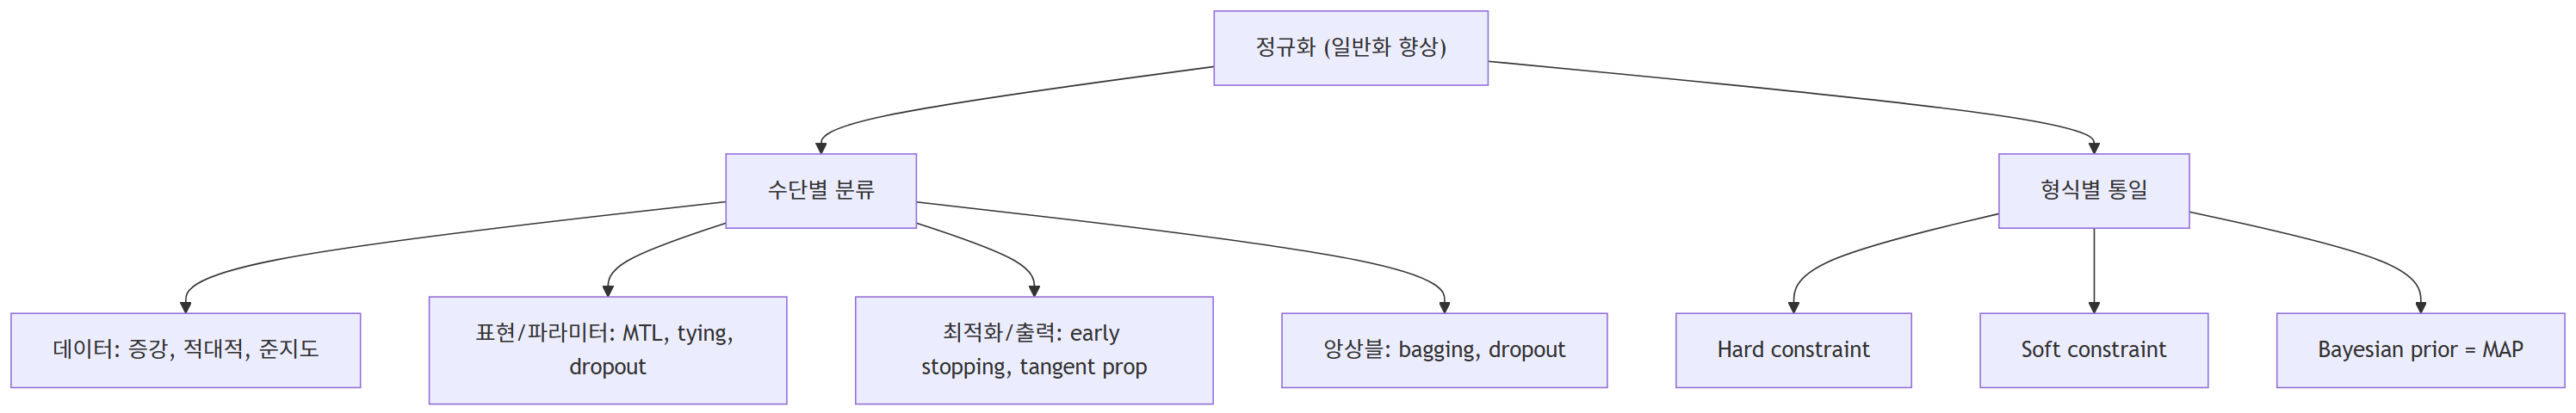
\includegraphics[width=19.51in,height=3.15in]{regularizer-for-dl_files/figure-latex/mermaid-figure-2.png}

\section{핵심 메시지}\label{uxd575uxc2ec-uxba54uxc2dcuxc9c0}

\begin{enumerate}
\def\labelenumi{\arabic{enumi}.}
\tightlist
\item
  모든 정규화는 식~\ref{eq-objective} 의 큰 틀 --- \textbf{Loss + 귀납적
  편향} --- 안에서 이해할 수 있다.
\item
  Hard / Soft / Bayesian-prior 세 형식은 KKT와 MAP을 통해 \textbf{서로
  등가}다(식~\ref{eq-map}).
\item
  겉보기에 다른 기법들이 동일한 효과로 수렴한다: 입력 노이즈·early
  stopping·tangent prop은 모두 어떤 의미에서 \textbf{함수의
  평탄성(자코비안 억제)}을 유도하고, bagging·dropout은 \textbf{분산 감소
  앙상블}로 묶인다.
\item
  무선통신의 직관 --- 다이버시티 결합(=bagging), 강건
  빔포밍(=adversarial), 반-블라인드 추정(=semi-supervised), 정상성
  가정(=parameter sharing) --- 이 정규화 전반을 관통한다.
\end{enumerate}

\begin{center}\rule{0.5\linewidth}{0.5pt}\end{center}

\chapter{부록: 실행 가능한 코드}\label{sec-appendix}

\section{\texorpdfstring{A. Bagging 분산 감소 (식~\ref{eq-bagging} 수치
검증)}{A. Bagging 분산 감소 (식~ 수치 검증)}}\label{a.-bagging-uxbd84uxc0b0-uxac10uxc18c-eq-bagging-uxc218uxce58-uxac80uxc99d}

\begin{Shaded}
\begin{Highlighting}[]
\ImportTok{import}\NormalTok{ numpy }\ImportTok{as}\NormalTok{ np}
\NormalTok{rng }\OperatorTok{=}\NormalTok{ np.random.default\_rng(}\DecValTok{0}\NormalTok{)}

\KeywordTok{def}\NormalTok{ ensemble\_var(k, v}\OperatorTok{=}\FloatTok{1.0}\NormalTok{, rho}\OperatorTok{=}\FloatTok{0.0}\NormalTok{, trials}\OperatorTok{=}\DecValTok{200\_000}\NormalTok{):}
    \CommentTok{"""k개 모델, 오차분산 v, 상관계수 rho일 때 평균오차의 분산을 추정."""}
\NormalTok{    c }\OperatorTok{=}\NormalTok{ rho }\OperatorTok{*}\NormalTok{ v}
    \CommentTok{\# 공분산행렬 Sigma: 대각 v, 비대각 c}
\NormalTok{    Sigma }\OperatorTok{=}\NormalTok{ np.full((k, k), c) }\OperatorTok{+}\NormalTok{ np.eye(k) }\OperatorTok{*}\NormalTok{ (v }\OperatorTok{{-}}\NormalTok{ c)}
\NormalTok{    L }\OperatorTok{=}\NormalTok{ np.linalg.cholesky(Sigma)}
\NormalTok{    eps }\OperatorTok{=}\NormalTok{ rng.standard\_normal((trials, k)) }\OperatorTok{@}\NormalTok{ L.T   }\CommentTok{\# 상관된 오차 샘플}
\NormalTok{    ebar }\OperatorTok{=}\NormalTok{ eps.mean(axis}\OperatorTok{=}\DecValTok{1}\NormalTok{)}
    \ControlFlowTok{return}\NormalTok{ ebar.var()}

\ControlFlowTok{for}\NormalTok{ k }\KeywordTok{in}\NormalTok{ [}\DecValTok{1}\NormalTok{, }\DecValTok{2}\NormalTok{, }\DecValTok{4}\NormalTok{, }\DecValTok{8}\NormalTok{, }\DecValTok{16}\NormalTok{]:}
\NormalTok{    emp }\OperatorTok{=}\NormalTok{ ensemble\_var(k, rho}\OperatorTok{=}\FloatTok{0.0}\NormalTok{)}
\NormalTok{    theory }\OperatorTok{=} \FloatTok{1.0} \OperatorTok{/}\NormalTok{ k            }\CommentTok{\# c=0이면 v/k}
    \BuiltInTok{print}\NormalTok{(}\SpecialStringTok{f"k=}\SpecialCharTok{\{}\NormalTok{k}\SpecialCharTok{:2d\}}\SpecialStringTok{ | empirical=}\SpecialCharTok{\{}\NormalTok{emp}\SpecialCharTok{:.4f\}}\SpecialStringTok{ | theory(v/k)=}\SpecialCharTok{\{}\NormalTok{theory}\SpecialCharTok{:.4f\}}\SpecialStringTok{"}\NormalTok{)}
\end{Highlighting}
\end{Shaded}

\begin{verbatim}
k= 1 | empirical=1.0024 | theory(v/k)=1.0000
k= 2 | empirical=0.5001 | theory(v/k)=0.5000
k= 4 | empirical=0.2499 | theory(v/k)=0.2500
k= 8 | empirical=0.1253 | theory(v/k)=0.1250
k=16 | empirical=0.0624 | theory(v/k)=0.0625
\end{verbatim}

비상관(\(\rho=0\))일 때 평균 오차 분산이 \(1/k\) 로 줄어드는 것을 확인할
수 있다. \(\rho\) 를 키우면 식~\ref{eq-bagging} 의
\(\frac1k v+\frac{k-1}{k}c\) 로 수렴한다.

\section{B. Dropout 순전파와 가중치
스케일링}\label{b.-dropout-uxc21cuxc804uxd30cuxc640-uxac00uxc911uxce58-uxc2a4uxcf00uxc77cuxb9c1}

\begin{Shaded}
\begin{Highlighting}[]
\ImportTok{import}\NormalTok{ numpy }\ImportTok{as}\NormalTok{ np}
\NormalTok{rng }\OperatorTok{=}\NormalTok{ np.random.default\_rng(}\DecValTok{1}\NormalTok{)}

\KeywordTok{def}\NormalTok{ dropout\_forward(h, p, training}\OperatorTok{=}\VariableTok{True}\NormalTok{, inverted}\OperatorTok{=}\VariableTok{True}\NormalTok{):}
    \CommentTok{"""Bernoulli dropout. p = drop 확률."""}
    \ControlFlowTok{if} \KeywordTok{not}\NormalTok{ training:}
        \ControlFlowTok{return}\NormalTok{ h }\ControlFlowTok{if}\NormalTok{ inverted }\ControlFlowTok{else}\NormalTok{ h }\OperatorTok{*}\NormalTok{ (}\DecValTok{1} \OperatorTok{{-}}\NormalTok{ p)     }\CommentTok{\# 표준 추론}
\NormalTok{    mask }\OperatorTok{=}\NormalTok{ (rng.random(h.shape) }\OperatorTok{\textgreater{}}\NormalTok{ p).astype(h.dtype)}
\NormalTok{    out }\OperatorTok{=}\NormalTok{ h }\OperatorTok{*}\NormalTok{ mask}
    \ControlFlowTok{if}\NormalTok{ inverted:}
\NormalTok{        out }\OperatorTok{/=}\NormalTok{ (}\DecValTok{1} \OperatorTok{{-}}\NormalTok{ p)        }\CommentTok{\# inverted dropout: 추론 무수정}
    \ControlFlowTok{return}\NormalTok{ out}

\NormalTok{h }\OperatorTok{=}\NormalTok{ np.ones(}\DecValTok{10\_000}\NormalTok{)           }\CommentTok{\# 모든 활성=1}
\NormalTok{p }\OperatorTok{=} \FloatTok{0.5}
\NormalTok{train\_out }\OperatorTok{=}\NormalTok{ dropout\_forward(h, p, training}\OperatorTok{=}\VariableTok{True}\NormalTok{, inverted}\OperatorTok{=}\VariableTok{True}\NormalTok{)}
\BuiltInTok{print}\NormalTok{(}\SpecialStringTok{f"훈련 시 평균 활성(inverted) ≈ }\SpecialCharTok{\{}\NormalTok{train\_out}\SpecialCharTok{.}\NormalTok{mean()}\SpecialCharTok{:.3f\}}\SpecialStringTok{  (목표 1.0)"}\NormalTok{)}
\BuiltInTok{print}\NormalTok{(}\SpecialStringTok{f"실제 drop된 비율 ≈ }\SpecialCharTok{\{}\NormalTok{(train\_out}\OperatorTok{==}\DecValTok{0}\NormalTok{)}\SpecialCharTok{.}\NormalTok{mean()}\SpecialCharTok{:.3f\}}\SpecialStringTok{  (목표 }\SpecialCharTok{\{}\NormalTok{p}\SpecialCharTok{\}}\SpecialStringTok{)"}\NormalTok{)}
\end{Highlighting}
\end{Shaded}

\begin{verbatim}
훈련 시 평균 활성(inverted) ≈ 1.009  (목표 1.0)
실제 drop된 비율 ≈ 0.495  (목표 0.5)
\end{verbatim}

inverted dropout은 훈련 시 기대 활성을 보존하므로 추론을 손대지 않아도
된다.

\section{\texorpdfstring{C. Early Stopping ↔ \(\ell_2\) 등가성
(식~\ref{eq-early-l2})}{C. Early Stopping ↔ \textbackslash ell\_2 등가성 (식~)}}\label{c.-early-stopping-ell_2-uxb4f1uxac00uxc131-eq-early-l2}

\begin{Shaded}
\begin{Highlighting}[]
\ImportTok{import}\NormalTok{ numpy }\ImportTok{as}\NormalTok{ np}

\CommentTok{\# 이차 손실 L(theta) = 0.5 (theta{-}theta*)\^{}T H (theta{-}theta*), H=diag(lams)}
\NormalTok{lams }\OperatorTok{=}\NormalTok{ np.array([}\FloatTok{5.0}\NormalTok{, }\FloatTok{1.0}\NormalTok{, }\FloatTok{0.1}\NormalTok{, }\FloatTok{0.01}\NormalTok{])   }\CommentTok{\# 곡률(고유값)}
\NormalTok{theta\_star }\OperatorTok{=}\NormalTok{ np.ones\_like(lams)}
\NormalTok{eps }\OperatorTok{=} \FloatTok{0.05}                                \CommentTok{\# 학습률}

\KeywordTok{def}\NormalTok{ gd\_solution(tau):}
    \CommentTok{\# 성분별 closed{-}form: theta\_tau = (1{-}(1{-}eps*lam)\^{}tau) theta*}
    \ControlFlowTok{return}\NormalTok{ (}\DecValTok{1} \OperatorTok{{-}}\NormalTok{ (}\DecValTok{1} \OperatorTok{{-}}\NormalTok{ eps }\OperatorTok{*}\NormalTok{ lams) }\OperatorTok{**}\NormalTok{ tau) }\OperatorTok{*}\NormalTok{ theta\_star}

\KeywordTok{def}\NormalTok{ l2\_solution(alpha):}
    \CommentTok{\# theta = lam/(lam+alpha) theta*}
    \ControlFlowTok{return}\NormalTok{ lams }\OperatorTok{/}\NormalTok{ (lams }\OperatorTok{+}\NormalTok{ alpha) }\OperatorTok{*}\NormalTok{ theta\_star}

\NormalTok{tau }\OperatorTok{=} \DecValTok{40}
\NormalTok{alpha\_equiv }\OperatorTok{=} \FloatTok{1.0} \OperatorTok{/}\NormalTok{ (tau }\OperatorTok{*}\NormalTok{ eps)          }\CommentTok{\# 식 (early{-}l2)}
\BuiltInTok{print}\NormalTok{(}\SpecialStringTok{f"tau=}\SpecialCharTok{\{}\NormalTok{tau}\SpecialCharTok{\}}\SpecialStringTok{, eps=}\SpecialCharTok{\{}\NormalTok{eps}\SpecialCharTok{\}}\SpecialStringTok{  {-}\textgreater{}  등가 alpha ≈ }\SpecialCharTok{\{}\NormalTok{alpha\_equiv}\SpecialCharTok{:.3f\}}\CharTok{\textbackslash{}n}\SpecialStringTok{"}\NormalTok{)}
\BuiltInTok{print}\NormalTok{(}\StringTok{"성분 | early{-}stopping |  L2(alpha\_equiv)"}\NormalTok{)}
\ControlFlowTok{for}\NormalTok{ i, (a, b) }\KeywordTok{in} \BuiltInTok{enumerate}\NormalTok{(}\BuiltInTok{zip}\NormalTok{(gd\_solution(tau), l2\_solution(alpha\_equiv))):}
    \BuiltInTok{print}\NormalTok{(}\SpecialStringTok{f"  }\SpecialCharTok{\{}\NormalTok{i}\SpecialCharTok{\}}\SpecialStringTok{  |    }\SpecialCharTok{\{}\NormalTok{a}\SpecialCharTok{:.4f\}}\SpecialStringTok{     |     }\SpecialCharTok{\{}\NormalTok{b}\SpecialCharTok{:.4f\}}\SpecialStringTok{"}\NormalTok{)}
\end{Highlighting}
\end{Shaded}

\begin{verbatim}
tau=40, eps=0.05  ->  등가 alpha ≈ 0.500

성분 | early-stopping |  L2(alpha_equiv)
  0  |    1.0000     |     0.9091
  1  |    0.8715     |     0.6667
  2  |    0.1817     |     0.1667
  3  |    0.0198     |     0.0196
\end{verbatim}

곡률이 큰 방향은 빠르게 \(\theta^*\) 로 수렴(둘 다 1에 가까움)하고,
곡률이 작은 방향은 억제되어 작은 값에 머문다 --- early stopping과
\(\ell_2\) 정규화가 같은 수축을 만든다.

\section{\texorpdfstring{D. FGSM 적대적 섭동
(식~\ref{eq-fgsm})}{D. FGSM 적대적 섭동 (식~)}}\label{d.-fgsm-uxc801uxb300uxc801-uxc12duxb3d9-eq-fgsm}

\begin{Shaded}
\begin{Highlighting}[]
\ImportTok{import}\NormalTok{ numpy }\ImportTok{as}\NormalTok{ np}

\KeywordTok{def}\NormalTok{ fgsm(grad\_x, eps):}
    \CommentTok{"""입력 그래디언트로부터 FGSM 섭동을 만든다."""}
    \ControlFlowTok{return}\NormalTok{ eps }\OperatorTok{*}\NormalTok{ np.sign(grad\_x)}

\NormalTok{x }\OperatorTok{=}\NormalTok{ np.array([}\FloatTok{0.2}\NormalTok{, }\OperatorTok{{-}}\FloatTok{0.5}\NormalTok{, }\FloatTok{0.9}\NormalTok{, }\OperatorTok{{-}}\FloatTok{0.1}\NormalTok{])}
\NormalTok{grad }\OperatorTok{=}\NormalTok{ np.array([}\FloatTok{1.3}\NormalTok{, }\OperatorTok{{-}}\FloatTok{0.4}\NormalTok{, }\FloatTok{0.8}\NormalTok{, }\OperatorTok{{-}}\FloatTok{2.1}\NormalTok{])   }\CommentTok{\# dJ/dx (가정)}
\NormalTok{x\_adv }\OperatorTok{=}\NormalTok{ x }\OperatorTok{+}\NormalTok{ fgsm(grad, eps}\OperatorTok{=}\FloatTok{0.1}\NormalTok{)}
\BuiltInTok{print}\NormalTok{(}\StringTok{"원본 x      :"}\NormalTok{, x)}
\BuiltInTok{print}\NormalTok{(}\StringTok{"적대적 x\_adv:"}\NormalTok{, np.}\BuiltInTok{round}\NormalTok{(x\_adv, }\DecValTok{3}\NormalTok{))}
\BuiltInTok{print}\NormalTok{(}\StringTok{"섭동 노름(∞):"}\NormalTok{, np.}\BuiltInTok{abs}\NormalTok{(x\_adv }\OperatorTok{{-}}\NormalTok{ x).}\BuiltInTok{max}\NormalTok{(), }\StringTok{"= eps"}\NormalTok{)}
\end{Highlighting}
\end{Shaded}

\begin{verbatim}
원본 x      : [ 0.2 -0.5  0.9 -0.1]
적대적 x_adv: [ 0.3 -0.6  1.  -0.2]
섭동 노름(∞): 0.10000000000000003 = eps
\end{verbatim}

\(\ell_\infty\) 제약 하에서 손실을 가장 키우는 섭동은 그래디언트의 부호
방향이며, 그 크기는 정확히 \(\epsilon\) 으로 균일하다.




\end{document}
